\documentclass[annual]{acmsiggraph}
\usepackage{wrapfig}
\usepackage{hyperref}
\title{X\texorpdfstring{\textsuperscript{2}}.-Toon: An Extended X-Toon Shader}

\author{Robert Wolfe\thanks{e-mail:robert\_wolfe@carleton.ca}\\Spencer Elliott\thanks{e-mail:spencer\_elliott@carleton.ca}}
\pdfauthor{Robert Wolfe, Spencer Elliott}

\keywords{xtoon, image processing, xna}

\begin{document}

\maketitle

\begin{abstract}

The X-toon shader ~\cite{BTM06a} extended classic cel shading from 1D shading textures to 2D textures. The second dimension ``corresponds to the desired `tone detail' ''. In this paper, we look to extend the initial offering of the X-Toon shader and develop new methods for calculating shading values and tone detail. Additionally, we extend the original shader to allow the use of model textures and transparency within a tone detail texture. This gives artists the tools to create new effects that were not possible with original X-Toon shader.

\end{abstract}

\keywordlist

\copyrightspace

\section{Introduction}
~\cite{BTM06a} extended the classical understanding of how to perform toon shading. A new dimension of tone detail can be used to create a desired level of abstraction. Our approach implements this technique, as well as extends it. We first developed a standard cel shader using ~\cite{CelShadingTut} as a starting point. Using models downloaded from ~\cite{TurboSquid}, we used a threshold of the dot product of the lighting vector and the surface normal to produce classic toon shading. An example can be seen in Figure~\ref{fig:toonshade}.

\begin{figure}[h]
	\centering
	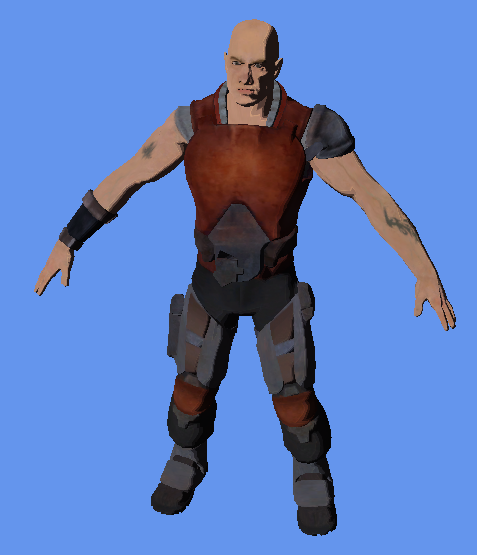
\includegraphics[width=2.5in]{images/classic_cel2}
	\caption{Classic Toon Shading}
	\label{fig:toonshade}
\end{figure}

A brief explanation of X-Toon is described in Section~\ref{sec:tonedetail}, our extensions in Section~\ref{sec:extensions}, and the results in Section~\ref{sec:results}. Discussion and future work are described in Section~\ref{sec:discussion} and finally the conclusion in Section~\ref{sec:conclusion}.

To make our program more interactive, we developed a GUI using the XNA GUI framework from ~\cite{Ruminate}. The controls allows the user to modify the parameters and enable/disable features.

\section{Tone Detail}
\label{sec:tonedetail}
\begin{wrapfigure}{r}{0.1\textwidth}
  \vspace{-20pt}
  \begin{center}
    
\includegraphics[width=0.1\textwidth]{images/xtoon_skin}
  \end{center}
  \caption{2D Texture.}
  \vspace{-10pt}
  \label{fig:2dtexture}
\end{wrapfigure}
X-Toon extends the regular toon shader by adding a second dimension to the texture. The x-axis remains as $N\cdot L$, where {\it{N}} is the surface normal and {\it{L}} is the light direction. The y-axis represents the level of detail. The higher up on the axis, the less detail is used. Conversely, the lower the y-axis value, the more detail. An example of a 2D tone detail texture used in this application can be seen in Figure~\ref{fig:2dtexture} (note the y-axis increases downward).

The method of computing the y-axis depends on an {\it{attribute map.}} The chosen attribute changes the level of detail, depending on its value. The original paper provided two possible attribute maps: distance and orientation. This paper deals exclusively with the distance attribute mapping. We provide an alternative mapping involving the angle between the camera {\it{look at}} vector and surface normal. 

In addition to providing an alternate attribute mapping, we also developed a new method for determining the amount of shading on a model. This method involves calculating direction vectors to each light from each vertex. The resulting vector can then be used to calculate the final shading amount.

\subsection{Distance}
\label{sec:distance}
As in the original X-Toon paper, one attribute map uses the focal distance of the vertex to the camera. The larger this distance, the less detail will be used, abstracting the model. The smaller this distance, the more detail used. Nothing was changed from the original paper. An example result can be seen in Figure~\ref{fig:distanceResult}, using a transparent tone detail texture (see Section~\ref{sec:transparency}).

\begin{figure}[h]
	\centering
	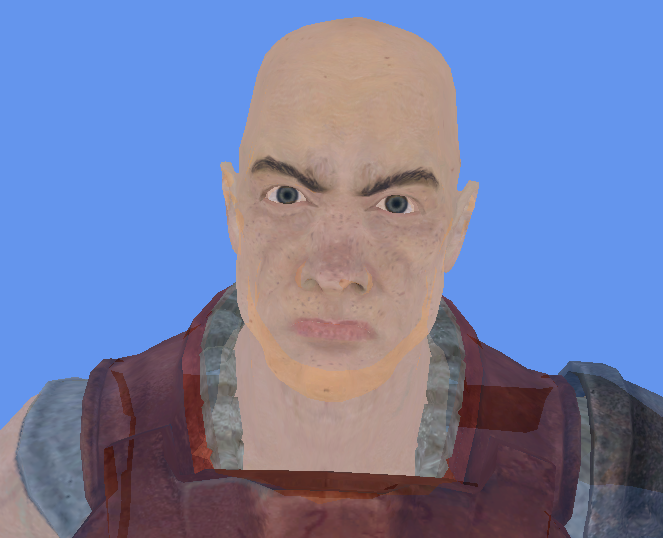
\includegraphics[width=2.5in]{images/distance_result}
	\caption{Parts of the model that are farther away are more transparent than closer areas.}
	\label{fig:distanceResult}
\end{figure}

\subsection{Angle}
\label{sec:angle}
We introduce a new attribute map based on the angles of the {\it{look at}} vector of the camera and the surface normal. The look at vector is the direction that the camera is pointed. The angle between the two vectors is calculated using Equation~\ref{eqn:angle}, which is derived from the formula for dot product.

\begin{equation}
\label{eqn:angle}
a = \cos^{-1}{(-LookAt \cdot Normal / |LookAt||Normal|)}
\end{equation}

The negative of the look at vector is used because it is pointed towards the surface (see Figure~\ref{fig:angle}). This value indicates what surfaces the camera is directly pointed at. The amount of detail used decreases as the angle between the look at vector and the surface normal approaches $180^\circ$, or when the surface is completely pointed away from the camera (or vice versa). As the angle approaches 0, more detail is used. An example result of this attribute map using a transparent tone detail texture can be seen in Figure~\ref{fig:angleResult}.

\begin{figure}[h]
	\centering
	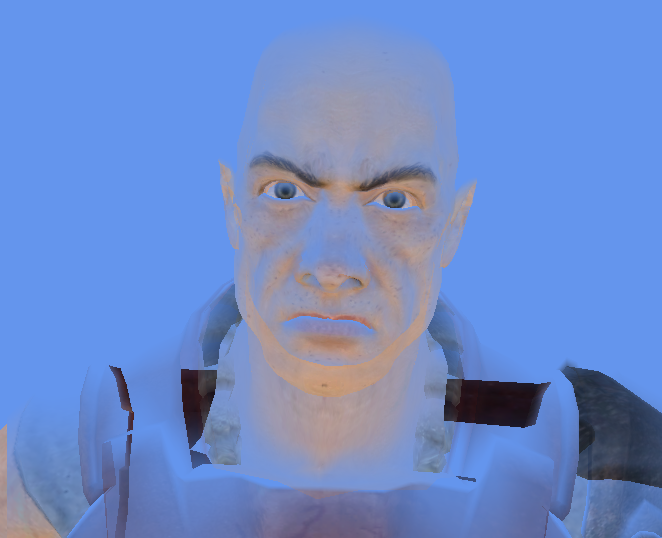
\includegraphics[width=2.5in]{images/angle_result}
	\caption{An example result generated using the angle attribute map. Surfaces that are facing the camera have more detail, while those angled away from the camera are more transparent.}
	\label{fig:angleResult}
\end{figure}

\begin{figure}[h]
	\centering
	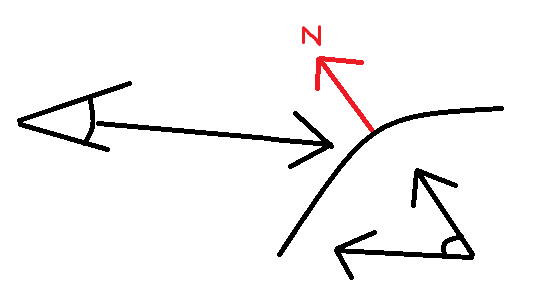
\includegraphics[width=1.5in]{images/angle}
	\caption{Diagram of the angle calculation using the camera (left)'s look at vector and the surface normal (right). The angle difference is calculated (bottom right) using Equation~\ref{eqn:angle}.}
	\label{fig:angle}
\end{figure}

\subsection{Light Direction}
\label{sec:light_dir}
We have developed a new method to determine the shading value on a model based on the lighting of a scene. Equation~\ref{eqn:light_dir} is used for determining the final vector. First, the direction from each light in {\it{Li}} to the vertex position, {\it{P}}, is calculated. These directions are then summed and a resulting direction vector is created. This direction is then normalized and the final detail vector, {\it{D}}, is determined. The same equation for determining the original shading value, $N\cdot L$, is used to determing the final shading value of the vertex. For the purpose of this method, {\it{N}} is represented by the final normalized direction vector, {\it{D}}. 

\begin{equation}
\label{eqn:light_dir}
D = normalize({\sum_{i=0}^{|Li|} Li[i] - P})
\end{equation}

\begin{figure}[h]
	\centering
	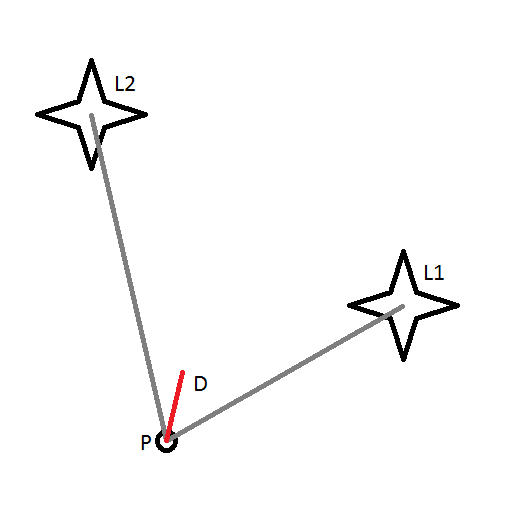
\includegraphics[width=1.5in]{images/light_detail}
	\caption{A diagram explaining the light direction attribute map.}
	\label{fig:lightDirection}
\end{figure}

\begin{figure}[h]
	\centering
	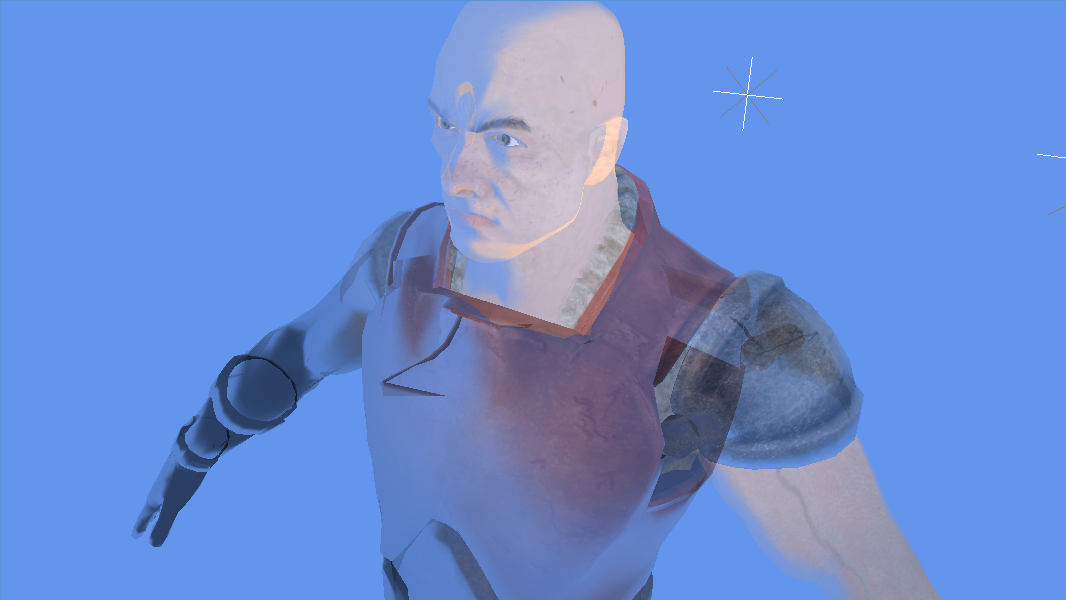
\includegraphics[width=3.0in]{images/light_directions}
	\caption{An example result of using the light direction attribute map.}
	\label{fig:lightDirectionResult}
\end{figure}

\section{Extensions to original X-Toon shader}
\label{sec:extensions}
We have extended the original shader offered in the X-Toon paper to increase the usability for various new effects. The first extension involves using colours from the original model's textures when calculating the final detail. The second extension allows for the use of transparency in both the tone texture and original model's textures to create a see-through effect for a model. 

\subsection{Texture blending}
\label{sec:blending}
We have added the ability to blend textures from a model into the calculation of the shading and tone detail. This technique gives artists the ability to retain the original look of the model while also applying the X-Toon effects. To achieve this effect, our shader first takes the pixel sample from the original texture. The shading and detail are determined using the calculations explained in previous sections and the final tone detail pixel is kept. To mix the colours of the original texture and the tone detail pixel, a simple multiplication of the {\it{RGB}} channels is performed. The resulting pixel is a blend of the original texture pixel and the sampled tone detail texture. Figure~\ref{fig:texturing} shows an example of a model with and without texture blending.

\begin{figure}[h]
	\centering
	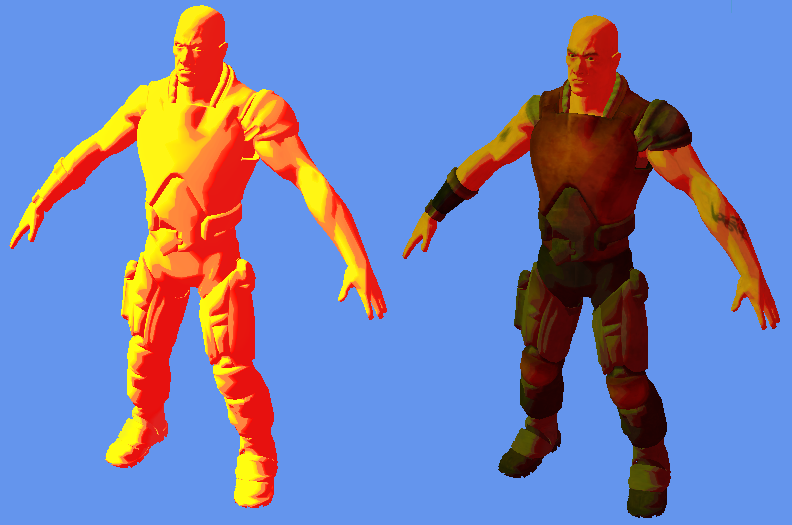
\includegraphics[width=3.0in]{images/textures}
	\caption{A model without and with original textures applied, respectively}
	\label{fig:texturing}
\end{figure}

\subsection{Texture transparency}
\label{sec:transparency}
The original X-Toon shader only supports the use of an opaque tone detail texture. We extend the shader to support the alpha channel of a tone detail texture to allow the use of transparency. Our method allows blending with original model's texture described in Section~\ref{sec:blending} or with the original method of using colour directly from the tone detail texture. An example of transparency in a tone detail texture can be seen in Figure~\ref{fig:transparency}. This example uses the tone detail texture shown in Figure~\ref{fig:transparent_tone}. The model is positioned so the detail is approximately at half. This gives each vertex an alpha of about 0.5 and the result is a model that is considerably transparent.

\begin{figure}[h]
	\centering
	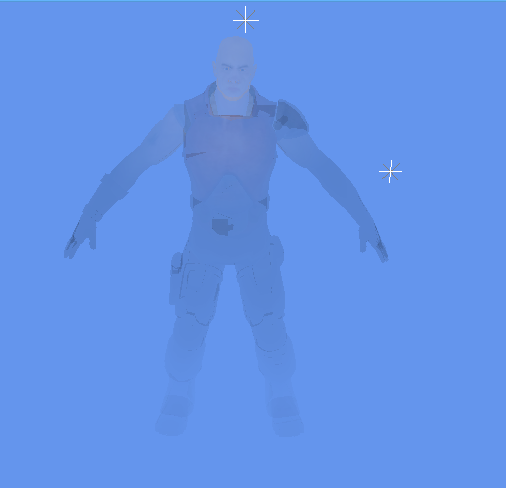
\includegraphics[width=2.5in]{images/transparency}
	\caption{Transparency affecting output}
	\label{fig:transparency}
\end{figure}

\begin{figure}[h]
	\centering
	
\includegraphics[width=1.5in]{images/xtoon_shading_alpha}
	\caption{Transparent tone detail texture. Note: the gray represents the transparency in the image.}
	\label{fig:transparent_tone}
\end{figure}

\section{Results}
\label{sec:results}
Using the new methods outlined in Sections~\ref{sec:angle},~\ref{sec:light_dir},~\ref{sec:blending}, and~\ref{sec:transparency}, we were able to develop new effects not possible with the original X-Toon shader. Figures~\ref{fig:hologram},~\ref{fig:stippleHatch1}, and~\ref{fig:stippleHatch2} use the same tone detail texture but result in different effects. This is achieved by mixing our techniques such as using the lighting directions outlined in~\ref{sec:light_dir} to create a hologram effect in Figure~\ref{fig:hologram}. Figure~\ref{fig:lightingResult} simulates self-shadowing. We use the textures from the original models and blend them with the tone detail texture found in Figure~\ref{fig:gradient}. This uses our texture blending technique described in Section~\ref{sec:blending}. Additionally, we were also able to have the self-shadowing effect interact with the lighting of the scene using the lighting directions as previously discussed.

\begin{figure*}[h]
 \centering
 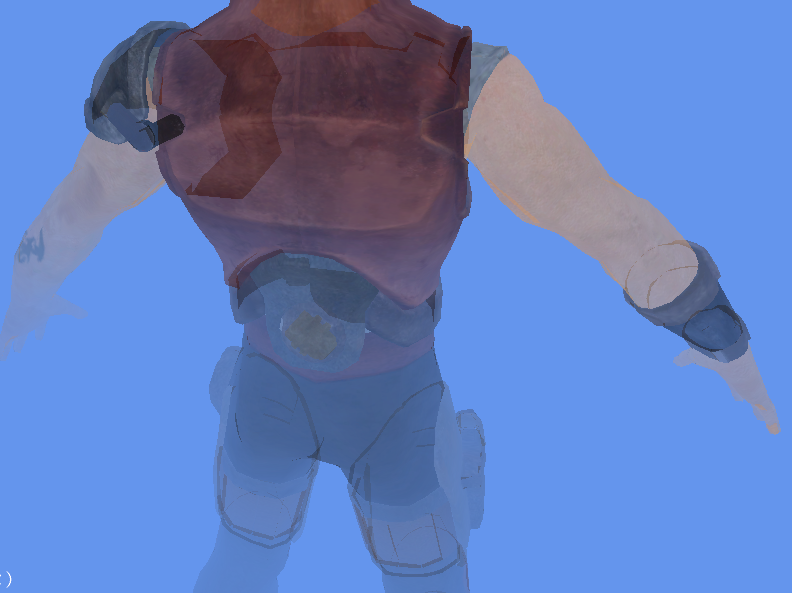
\includegraphics[width=5.5in]{images/alpha_issues}
 \caption{Issues with alpha blending. The vertices on the front of the model can still be seen.}
 \label{fig:alpha_issue}
\end{figure*}

\begin{figure*}[h]
	\centering
	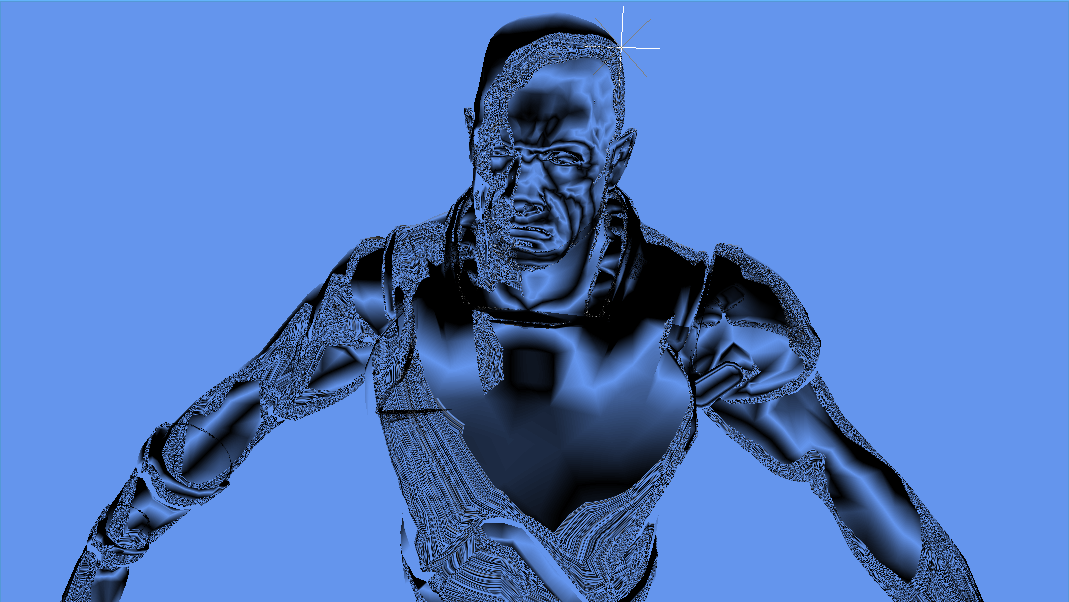
\includegraphics[width=5.5in]{images/hologram}
	\caption{A hologram-like result. Textures from the model are not used, and a noise texture is used. As the y-axis on the 2D Texture decreases, the amount of noise increases.}
	\label{fig:hologram}
\end{figure*}

\begin{figure*}[h]
	\centering
	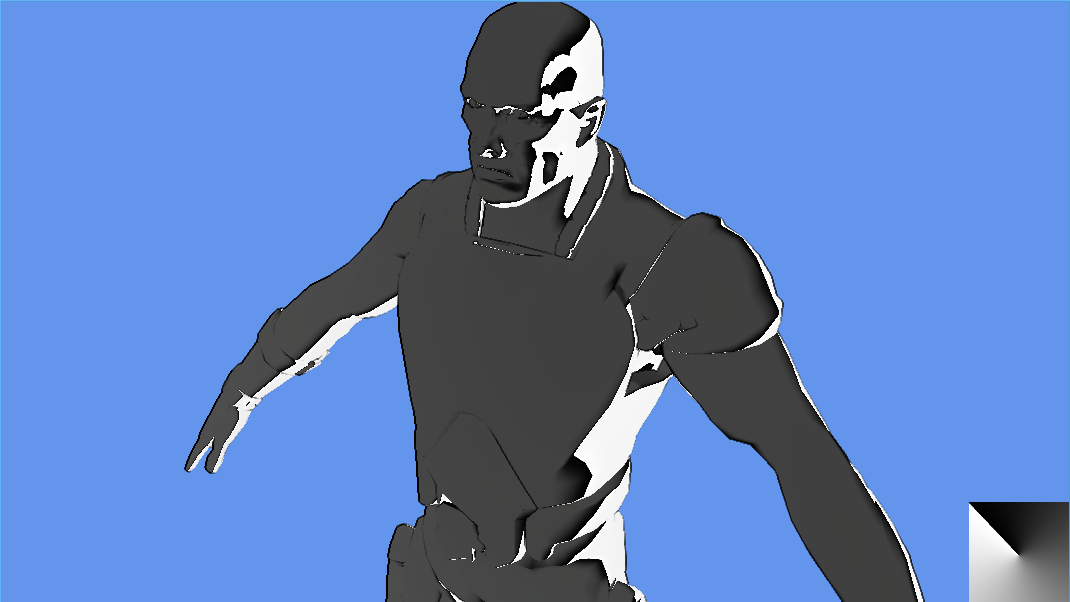
\includegraphics[width=5.5in]{images/inverse_lighting}
	\caption{Inverse Lighting result. The model appears to be lit from the opposite direction but no lighting variables or directions have been altered.}
	\label{fig:inverseLighting}
\end{figure*}

\begin{figure*}[h]
	\centering
	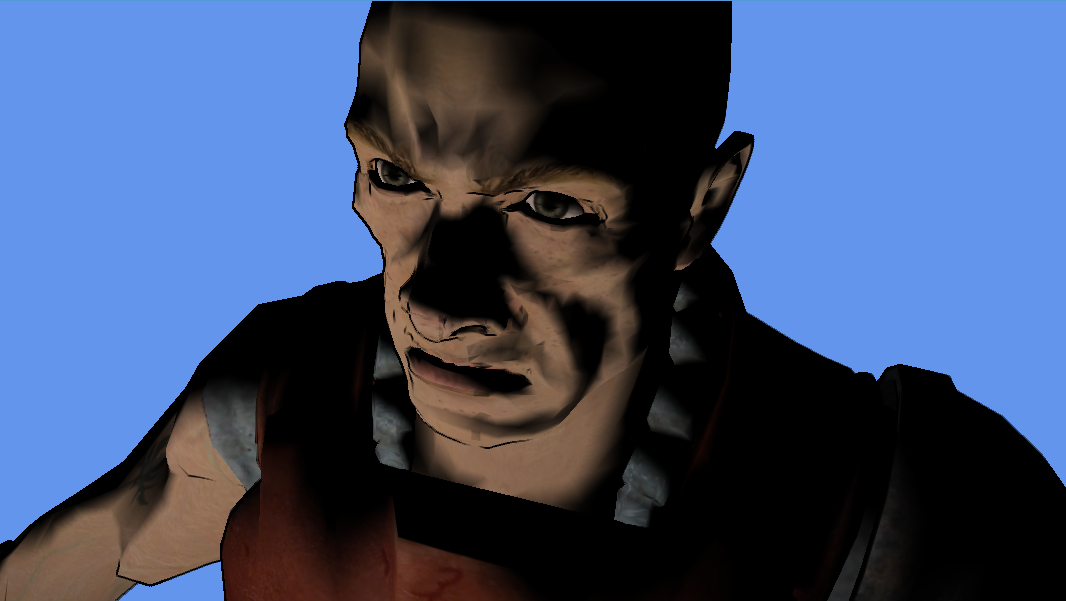
\includegraphics[width=5.5in]{images/lighting}
	\caption{Lighting result. The model appears to self-shadow itself using only the tone detail texture.}
	\label{fig:lightingResult}
\end{figure*}

\begin{figure}[h]
	\centering
	
\includegraphics[width=1.5in]{images/xtoon_shading_gradient}
	\caption{Tone texture for lighting. This gives the effect of self-shadowing on a model, especially when combined with lighting directions.}
	\label{fig:gradient}
\end{figure}

\begin{figure*}[h]
	\centering
	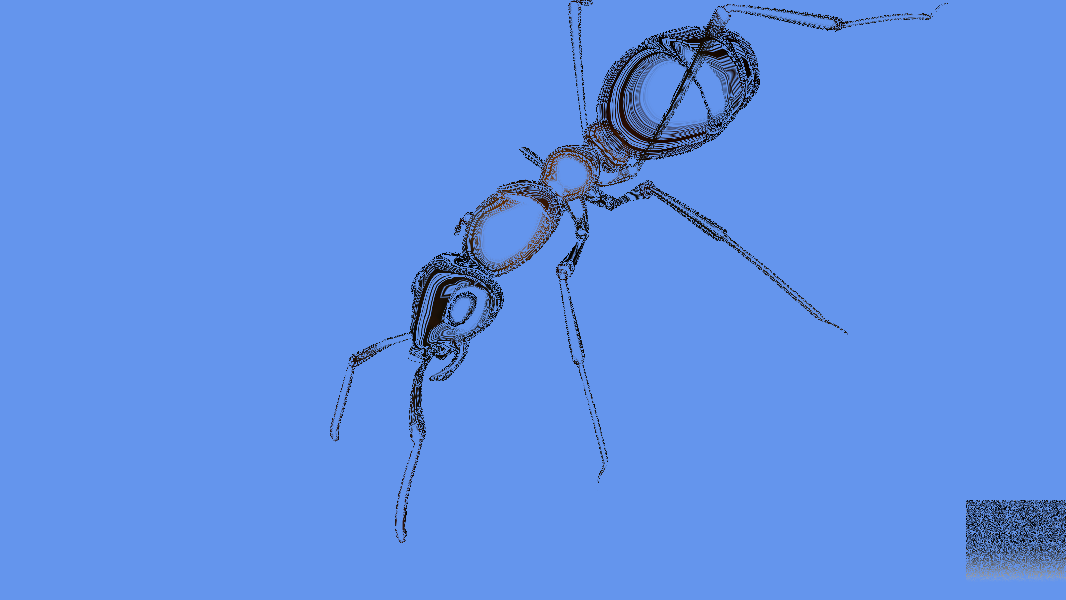
\includegraphics[width=5.5in]{images/stipple-hatch-result1}
	\caption{A stipple and hatching-like result of an ant. A noise 2D texture was used. Vertices closer to the camera were more noisy, while those further away were transparent. The gaster of the ant looks like it was done through hatching, while the rest of its body looks like it was done through stipppling.}
	\label{fig:stippleHatch1}
\end{figure*}

\begin{figure*}[h]
	\centering
	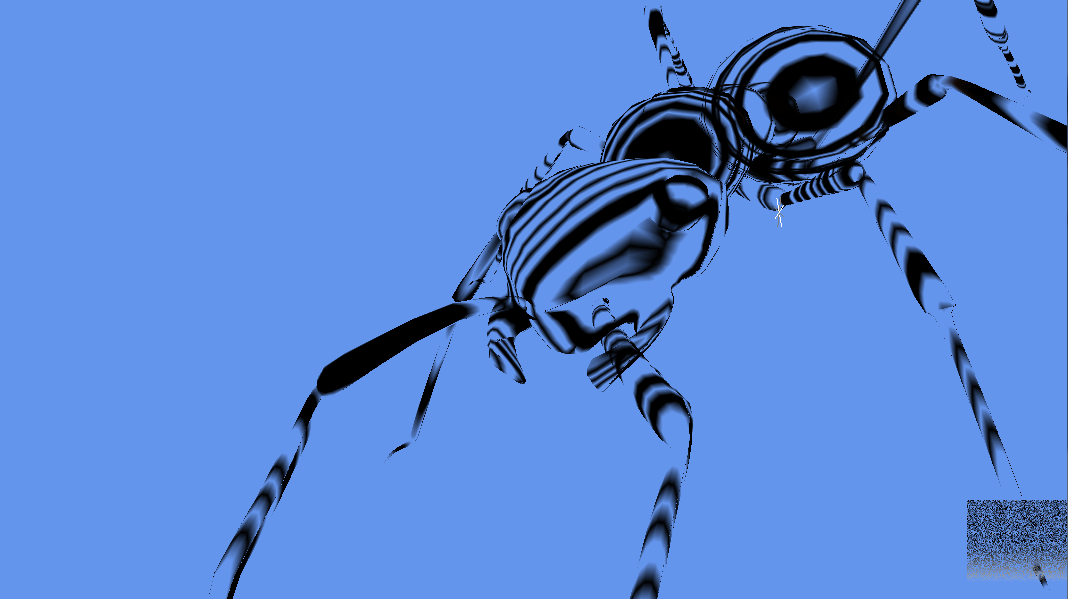
\includegraphics[width=5.5in]{images/stipple-hatch-result2}
	\caption{A hatching-like result of an ant. A noise 2D texture was used. Vertices closer to the camera were more noisy, and looked more like hatches, while those further away were transparent.}
	\label{fig:stippleHatch2}
\end{figure*}

\begin{figure*}[h]
  \centering
  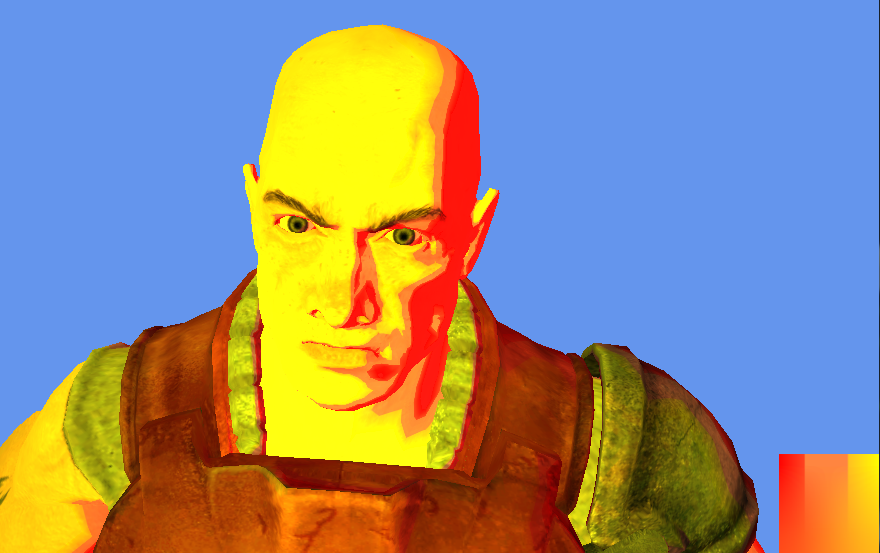
\includegraphics[width=5.5in]{images/test}
  \caption{Using a 2D texture from the original paper, we create a unique result by mixing the model's texture colors and the colors from the tone detail texture.}
\end{figure*}

\begin{figure*}[h]
 \centering
 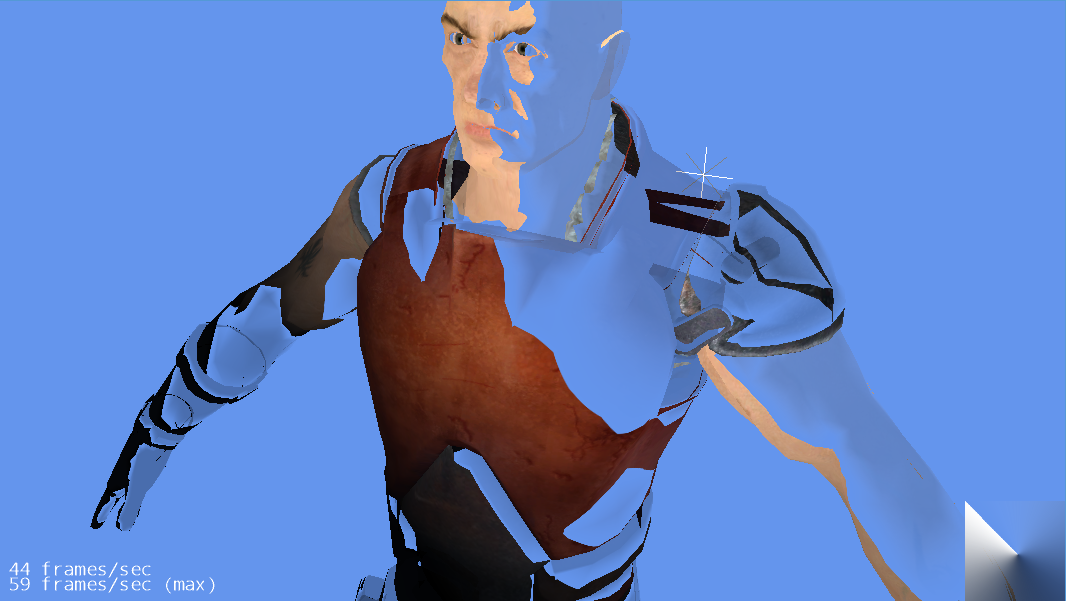
\includegraphics[width=5.5in]{images/dissolve}
 \caption{A dissolving effect. Using the lighting directions and the generated tone detail texture we were able to give the impression of the model dissolving in and out of view.}
 \label{fig:dissolve}
\end{figure*}

\begin{figure*}[h]
 \centering
 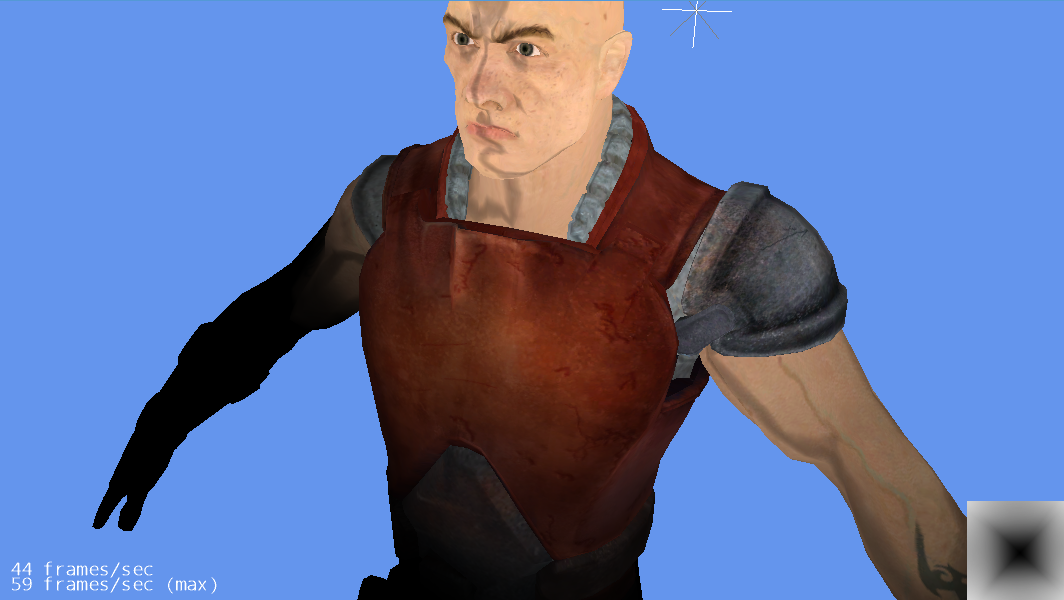
\includegraphics[width=5.5in]{images/metallic}
 \caption{A metallic sheen effect. The light directions give the model a metallic look as the tone detail texture reacts to new directions.}
 \label{fig:metallic}
\end{figure*}


\section{Discussion and Future Work}
\label{sec:discussion}
We have presented multiple extensions to the original X-Toon shader developed by  ~\cite{BTM06a}.  In order to retain the speed of the X-Toon shader, we attempted to minimize the complexity of the code executed in our shaders. The code added for transparency and texture blending, as well as our new calculations for tone detail, resulted in minimal performance reductions. To investigate the performance of our code, we calculated the frames per second (FPS) and removed the fixed time step. Two nVidia Geforce GTX 470 in SLI mode and an Intel i5 processor on Windows 8 were used for the calculation. The values found in Table~\ref{tab:fps} show the resulting FPS of the new methods introduced in this paper compared to the original X-Toon shader. We have concluded that our results are within a suitable error threshold and do not hinder the original shader, performance-wise. This data does not take into account any errors that may have arisen from factors such as the operating system and background applications affecting the outcome. 
In the two next sections, we will discuss future work that can be done to improve upon our methods outlined in this paper. First, we describe issues with alpha blending and a possible solution. Second, we discuss the effect of adding multiple lights to a scene and their performance implications.

\begin{table}
	\centering
	\caption{Frames per second (FPS) of each new technique compared to original X-Toon shading}
	\label{tab:fps}
	\begin{tabular}{cccc}
		\hline
    		Method  & FPS (avg) & FPS (max) & \% difference \\
		\hline\hline \\
    		Original X-Toon  & 1348 & 1420  & -                  \\
    		Light Direction & 1323 & 1435 & -1.85                \\
		Angle & 1354 & 1447 & 0.45 \\
		Texture Blending & 1347 & 1430 & -0.07 \\
		Transparency & 1345 & 1419 & -0.22 \\
		\hline
	\end{tabular}
\end{table}

\subsection{Alpha blending correction}
Figure~\ref{fig:alpha_issue} demonstrates issues with alpha blending when using a tone detail texture with transparency. When a model is rendered, the polygons hidden from the camera's view should not be rendered. Unfortunately, we are using alpha blending while rendering which results in these polygons being visible. In future works, a different technique should be used to calculate whether a pixel should overwrite the original pixel colour based on the depth and position of the polygon. If a polygon is fully covered and has a deeper depth value, it should be excluded from the scene. The alpha channel should only be considered in the output pixel value returned from the pixel shader.

\subsection{Lighting model}
The most significant result pertains to the light direction technique outlined in Section~\ref{sec:light_dir}. The calculated difference from Table~\ref{tab:fps} resulted in a 1.85\% performance drop compared to the original X-Toon shader. This is the result of only using two lights for the detail calculation. This performance drop will only increase as more lights are added to a scene. When calculating the light direction, the shader loops over each light in the scene resulting in a linear complexity of $O(n)$. In future works, a different lighting model should be developed to interact with the shader. The method we have developed is not viable for complex scenes and is limited to a very small amount of lights before it begins to reduce performance significantly. 

\subsection{Animated tone detail texture}
We also discussed the possibility of using an animated tone detail texture in lieu of a static image. This could create many new effects such as hologram noise and colour shifting without the need to change tone detail or shading values. Future works should investigate the use of an animated tone detail texture and devise new effects that can be generated with this method.

\section{Conclusion}
\label{sec:conclusion}
We have presented multiple extensions to the original X-Toon shader outlined by ~\cite{BTM06a}. Our texture blending method allow for artists to blend the original textures from a model with the calculated tone detail. Additionally, we have extended the original tone detail textures to allow transparency which creates see-through effects for a model. We have also outlined a new method for determining the shading based on lighting direction. Finally, a new method was created to calculate detail based on the the angle between a camera's look at vector and a model's surface normal. Combining the techniques outlined in this paper, a designer can achieve many new effects not possible in the original X-Toon shader.

\bibliographystyle{acmsiggraph}
\bibliography{paper}
\end{document}
